\documentclass[11pt]{article}

\usepackage{graphicx} % gere les images 
\usepackage[utf8]{inputenc} % pour les accents
\usepackage{hyperref} % pour les hyperliens
\usepackage[french]{babel} % langue fr
\usepackage{geometry} % pour les marges
\usepackage{listings} % pour le code
\usepackage{color}
\usepackage{enumitem} % permet de changer les listes a puces avec des rond
\usepackage{float}  % pour forcer les images a ce placer ou l'on veux avec l'option H
%\usepackage{here}  % pareil que float

\title{L'affichage de l'enveloppe convexe dans le plan euclidien usuel} 
\author{Armen Mahmedov, Aurelien Patru} 
\date{\today} 

\title{L'affichage de l'enveloppe convexe dans le plan euclidien usuel} 
\author{Armen Mahmedov, Aurelien Patru} 
\date{\today} 


\hypersetup {
	colorlinks=true,
	linkcolor=black,
	urlcolor=red,
	citecolor=green,
	pdftitle={Initiation aux outils de simulation réseaux avec NS-2},
	pdfauthor={Armen,Aurelien},
	pdfsubject={simulation réseau avec NS-2},
	pdfkeywords={NS-2, réseau, nam, esirem, tcp, udp, }
}


% ################### Configuration partie code ########################### %
\definecolor{darkWhite}{rgb}{0.94,0.94,0.94}
\lstset{
	aboveskip=3mm,
	belowskip=-2mm,
	%backgroundcolor=\color{darkWhite},
	basicstyle=\footnotesize\ttfamily,
	breakatwhitespace=false,
	breaklines=true,
	captionpos=b,
	deletekeywords={...},
	escapeinside={\%*}{*)},
	extendedchars=true,
	keepspaces=true,
	%keywordstyle=\color{blue},
	literate=
	{²}{{\textsuperscript{2}}}1
	{⁴}{{\textsuperscript{4}}}1
	{⁶}{{\textsuperscript{6}}}1
	{⁸}{{\textsuperscript{8}}}1
	{€}{{\euro{}}}1
	{é}{{\'e}}1
	{è}{{\`{e}}}1
	{ê}{{\^{e}}}1
	{ë}{{\¨{e}}}1
	{É}{{\'{E}}}1
	{Ê}{{\^{E}}}1
	{û}{{\^{u}}}1
	{ù}{{\`{u}}}1
	{â}{{\^{a}}}1
	{à}{{\`{a}}}1
	{á}{{\'{a}}}1
	{ã}{{\~{a}}}1
	{Á}{{\'{A}}}1
	{Â}{{\^{A}}}1
	{Ã}{{\~{A}}}1
	{ç}{{\c{c}}}1
	{Ç}{{\c{C}}}1
	{õ}{{\~{o}}}1
	{ó}{{\'{o}}}1
	{ô}{{\^{o}}}1
	{Õ}{{\~{O}}}1
	{Ó}{{\'{O}}}1
	{Ô}{{\^{O}}}1
	{î}{{\^{i}}}1
	{Î}{{\^{I}}}1
	{í}{{\'{i}}}1
	{Í}{{\~{Í}}}1,
	morekeywords={*,...},
	framexleftmargin=16pt,
	framextopmargin=3pt,
	framexbottommargin=6pt,
	frame=td,
	numbers=left,    % numerotation
	numbersep=10pt,
	numberstyle=\tiny\color{black},
	stepnumber=1,
	rulecolor=\color{black},
	showspaces=false,
	showstringspaces=false, % don't mark spaces in strings
	showtabs=false,
	%stringstyle=\color{red},
	title=\lstname,
	keywordstyle=\color{red}\bfseries, 
 	commentstyle=\color{blue}\textit,
 	stringstyle=\color{cyan}\ttfamily,
 	tabsize=2,
 	frame=single % or td
}

% Pour changer les listings en Code
\renewcommand\lstlistingname{Code}
\renewcommand\lstlistlistingname{Codes}

\setlist[itemize]{label=\textbullet} % pour tous les itemize changer le tiret avec un rond


\begin{document}

\begin{titlepage}
	\newcommand{\HRule}{\rule{\linewidth}{0.2mm}}     
            
	\begin{figure}[t]
		\begin{minipage}{0.5\textwidth}\large
			\begin{flushleft}
				
\includegraphics[width=0.7\textwidth]{assets/logoEsirem.jpg}
			\end{flushleft}
		\end{minipage}
		\begin{minipage}{0.5\textwidth}\large
			\begin{flushright}
			
\includegraphics[width=0.6\textwidth]{assets/logoUb.jpg}
			\end{flushright}
		\end{minipage}
	\end{figure}
	\textsc{ \\[1cm]}
     
     
	\begin{center}
	\HRule \\
	{\Large   
		Initiation aux outils de simulation réseaux avec NS-2
	}
	\HRule
	\\[0.5cm]
	{\large Compte rendu tp reseau \\}
   \end{center}

	\begin{figure}[h]
		\begin{center}
			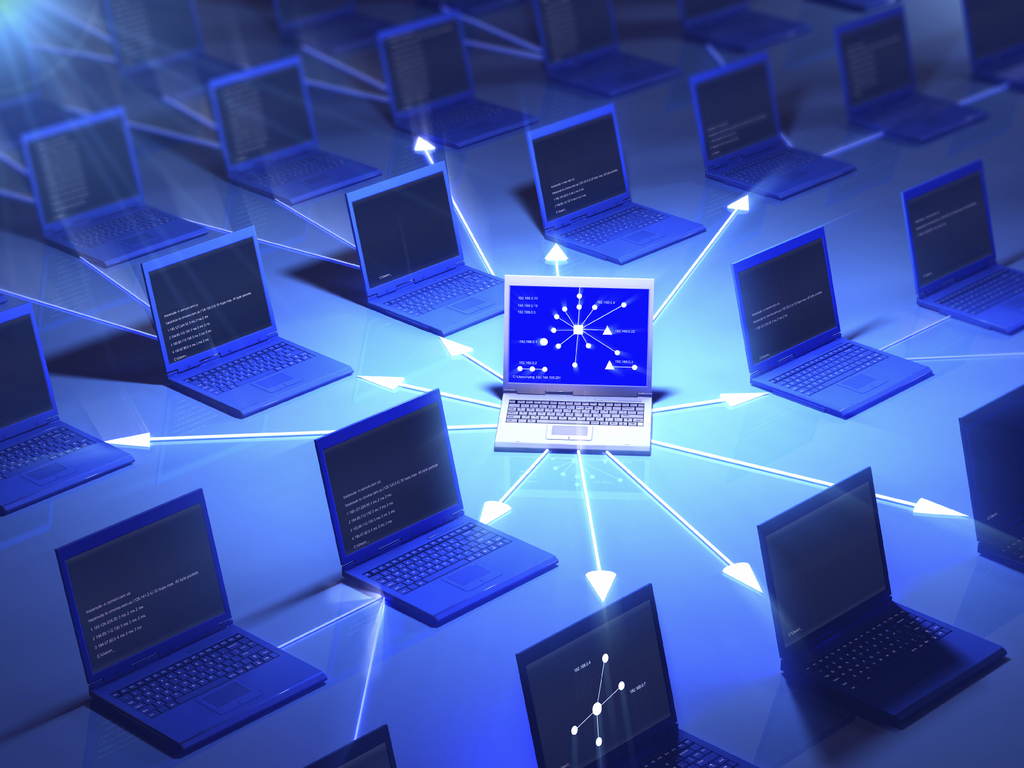
\includegraphics[width=0.4\textwidth]{assets/main.jpg}
		\end{center}
	\end{figure}
        
	\vfill 
	\begin{center}
        \textsc{\large
        	ESIREM \\
			École Supérieure d'Ingénieurs de Recherche en Matériaux et en Infotronique\\       	
			[2cm]
		}
	\end{center}

	\begin{minipage}{0.5\textwidth}
		\begin{flushleft} \large
			\emph{Auteurs:}\\
			Armen Mahmedov \\
			Aurélien Patru
		\end{flushleft}
	\end{minipage}
	~
	\begin{minipage}{0.5\textwidth}
		\begin{flushright}\large
			\emph{Professeurs :} \\
			Nader Mbarek \\
			Ahmad Khalil
		\end{flushright}
	\end{minipage}
        
\end{titlepage}
  
% saut de page  ou   ~ \pagebreak 
\newpage
\strut
\newpage

%------------------------
%     Table des matieres
%------------------------
\tableofcontents

\pagebreak

%------------------------
%    Table des figures
%------------------------
\listoffigures

\pagebreak


\section*{Introduction}
\addcontentsline{toc}{section}{Introduction}
Introduction générale 

\pagebreak


% Partie 1
\section{TP 1: Découvert de NS-2 et nam}
[introduction de la partie] **** dire le but du tp  *****

\subsection{Exercice 1: Simulation d'une topologie simple a deux noeuds avec un lien direct}

Dans un premier temps le but est de compléter le script fournis pour comprend se familiariser avec le language et comprendre son fonctionnent

\subsubsection{Compléter le script}
\noindent 
Pour créer deux nœuds on utilise la commande \textbf{set}. Pour cela on peut soit créer les nœuds un par un soit le faire a l'aide d'un boucle for :

\begin{lstlisting}[language=tcl, numbers=none, framexleftmargin=0pt, framextopmargin=0pt, framexbottommargin=0pt]
set NodeNb 2
for {set i 0} {$i<$NodeNb} {set i [expr $i+1]} {set n($i) [$ns node]}
\end{lstlisting}

\noindent % pour ne pas faire d'alinea
Pour relier les deux nœuds on utilisera les paramètres suivants:
\begin{itemize}
	\item lien duplex de capacité 1MB
	\item temps de propagation de 10ms
	\item file d'attente de type DropTail
\end{itemize}

\begin{lstlisting}[language=tcl, numbers=none, framexleftmargin=0pt, 	framextopmargin=0pt, framexbottommargin=0pt]
$ns duplex-link $n(0) $n(1) 1Mb 10ms DropTail
\end{lstlisting}

\noindent
Créer un agent UDP et l'attacher a n0. Ici la variable udp est une instance de la classe UDP qui hérite de la classe Agent

\begin{lstlisting}[language=tcl, numbers=none, framexleftmargin=0pt, 	framextopmargin=0pt, framexbottommargin=0pt]
set udp [new Agent/UDP]
#atacher l'aplication udp au noeud 0
$ns attach-agent $n(0) $udp 
\end{lstlisting}


Ensuite il faut créer une source de trafic CBR (\textit{constant bit rate}) avec les paramètres suivant:
\begin{itemize}
	\item taille des paquets de 500 octets
	\item intervalle de transmission de paquets de 0.005s
\end{itemize}

\begin{lstlisting}[language=tcl, numbers=none, framexleftmargin=0pt, 	framextopmargin=0pt, framexbottommargin=0pt]
#creattion d'un source de trafique
set cbr [new Application/Traffic/CBR]
$cbr set packetSize_ 500bytes
$cbr set interval_ 0.005s
\end{lstlisting}

\noindent
Après avoir créer la source CBR, il faut maintenant le connecter a l'agent UDP avec la commande \textbf{attach-agent}
\begin{lstlisting}[language=tcl, numbers=none, framexleftmargin=0pt, 	framextopmargin=0pt, framexbottommargin=0pt]
#connecter le cbr a l'agent UDP
$cbr attach-agent $udp
\end{lstlisting}

\noindent

Ensuite on doit créer l'agent null pour la réception des paquets dans le noeud 1 et connecter les deux agents Null et UDP
\begin{lstlisting}[language=tcl, numbers=none, framexleftmargin=0pt, 	framextopmargin=0pt, framexbottommargin=0pt]
#creation de l'agent null
set agentNull [new Agent/Null]
#atacher l'agent null au noeud 1
$ns attach-agent $n(1) $agentNull 
#connecter l'agent null et l'agent udp
$ns connect $udp $agentNull 
\end{lstlisting}

Il ne reste plus qu'à déclencher le trafic CBR à t=1s et l’arrêter à t=4.5s. Pour finir on doit arrêter la simulation après 5s. 
\begin{lstlisting}[language=tcl, numbers=none, framexleftmargin=0pt, 	framextopmargin=0pt, framexbottommargin=0pt]
#declancher le trafic cbf
$ns at 1 "$cbr start"
$ns at 4.5 "$cbr stop"
#Appeler la procédure de terminaison apres un temmps t 
$ns at 5.0 "finish"
#Executer la simulation
$ns run
\end{lstlisting}



\noindent
Le script en entier se trouve dans l'annexe 1 ( pas encore fait le faire plus tard)

\subsubsection{Visualisation de la simulation a l'aide de NAM}
Une fois le script complété on ouvre un terminal et on tape la commande \textbf{ns exercice1.tcl} pour compiler et lancer l'interface graphique nam que l'on peut voir dans la figure \ref{namVisu}. Cette commande crée aussi un fichier out.nam qui a été définit plus haut dans le script, plus tard si on veux revoir la simulation avec nam il suffira de lancer la commande \textbf{nam out.nam}


\subsubsection{Découvert des fonctionnalités de NAM}
L'utilitaire s'ouvre sur l'interface présentée en Figure \ref{namVisu}. Pour mieux comprendre le fonctionnement de nam on va détailler les différents parties présent en rouge sur la figure.

\begin{figure}[H]
	\begin{center}
		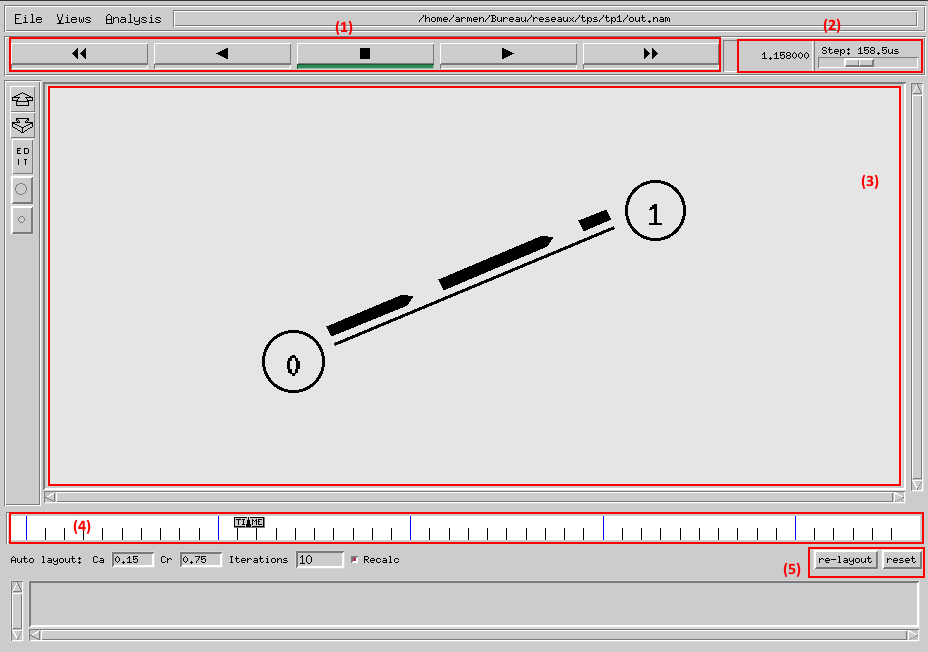
\includegraphics[width=0.7\textwidth]{assets/tp1/nam-visualisation1.png}
	\end{center}
	\caption{Interface nam pour la visualisation de la simulation}
	\label{namVisu}
\end{figure}

\noindent
(1) Sert a contrôler le déroulement la simulation \\
(2) Sert a visualiser le temps de la simulation et permet de contrôler sa vitesse\\
(3) Interface graphique ou la simulation se passe \\
(4) Permet de visualiser l'avancement de la simulation par rapport a la duré de la simulation et permet de se rendre directement un moment de la simulation\\
(5) Permet de changer la disposition des nœuds dans le cas ou les liens se croisent ou de reset la disposition des liens\\


********** Mettre les images présent dans le dossier TP1 **************************

\subsubsection{Utilisation graphique de NAM}


\begin{figure}[H]
	\begin{center}
		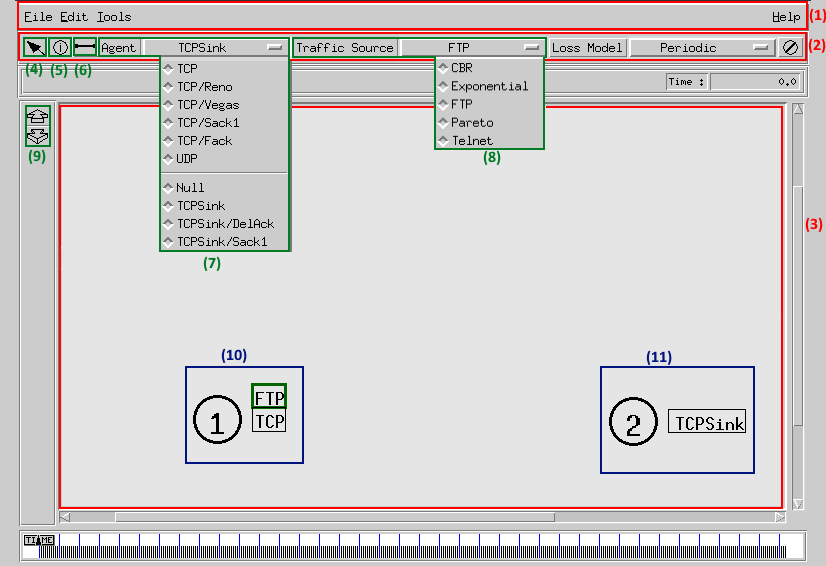
\includegraphics[width=0.8\textwidth]{assets/tp1/explicationNam.png}
	\end{center}
	\caption{L'interface graphique nam}
	\label{namExplcation}
\end{figure}

\subsection{Exercice 2: Fonctionnement TCP vs UDP}



[conclusion de la partie]


\pagebreak
% Partie 2
\section{TP 2: Protocole de routage de type Vecteur distance et Etat de liens}
[introduction de la partie]

\subsection{Exercice 1: Comparaison des deux protocoles de routage}


\subsection{Exercice 2: Routage et contrôle de congestion TCP}

[conclusion de la partie]

\pagebreak
% Partie 3
\section{TP 3: Utilisation de xgraph et NS-2 pour visualiser les performances d'un réseau}
[introduction de la partie]

\subsection{Sous-partie 1}

[conclusion de la partie]




\pagebreak
\section*{Conclusion}
\addcontentsline{toc}{section}{Conclusion}
[Conclusion générale]


\pagebreak
\section*{Annexes}
\addcontentsline{toc}{section}{Annexes}





[exemple de code TCL a effacer]


\begin{lstlisting}[language=tcl, caption={exemple Code TCL}]
#Création d'une instance de l'objet Simulator
set ns [new Simulator]

#Ouvrir le fichier trace pour nam
set nf [open out.nam w]
$ns namtrace-all $nf

#Définir la procedure de terminaison de la simuatation
proc finish {} {
	global ns nf
	$ns flush-trace
	#fermer le fichier trace
	close $nf
	#Exectuer le nam avec en entrée le fichier trace
	exec nam out.nam &
	exit 0
}

#Insérer votre code
set NodeNb 2
for {set i 0} {$i<$NodeNb} {set i [expr $i+1]} {set n($i) [$ns node]}
#connecter les deux noeuds
$ns duplex-link $n(0) $n(1) 1Mb 10ms DropTail
set udp [new Agent/UDP]
#atacher l'aplication udp au noeud 0
$ns attach-agent $n(0) $udp 
#creattion d'un source de trafique
set cbr [new Application/Traffic/CBR]
$cbr set packetSize_ 500bytes
$cbr set interval_ 0.005s
#connecter le cbr a l'agent UDP
$cbr attach-agent $udp

#creation de l'agent null
set agentNull [new Agent/Null]
#atacher l'agent null au noeud 1
$ns attach-agent $n(1) $agentNull 
#connecter l'agent null et l'agent udp
$ns connect $udp $agentNull 
#declancher le trafic cbf
$ns at 1 "$cbr start"
$ns at 4.5 "$cbr stop"

#Appeler la procédure de terminaison apres un temmps t 
$ns at 5.0 "finish"

#Executer la simulation
$ns run

\end{lstlisting} 






\end{document}
